\documentclass{beamer}
\usetheme{default}

\usepackage{amsmath, amsfonts}
\usepackage{color}
\usepackage{amssymb}
\usepackage{mathrsfs}
\usepackage{multicol}
\usepackage{fontspec}
\usepackage{cancel}
\usepackage{pgfplots}
\usepackage{booktabs}
\usefonttheme[onlymath]{serif}
\usepackage{tikz}
\usetikzlibrary{shapes.geometric, arrows}

\newcommand{\hbo}{\hat{\beta}^{OLS}}
\newcommand{\X}{\mathbf{X}}
\newcommand{\Y}{\mathbf{Y}}



\title{An Introduction to Regularized Regression}
\subtitle{Machine Learning and Causal Inference}
\author{Susan Athey}

\begin{document}
	
\begin{frame}
\titlepage
\end{frame}

\begin{frame}{What we do in Econometrics: The Case of Regression}
	\begin{itemize}
		\item specify a model:
		$$Y_i=f\left( X_i\right) +\varepsilon_i=X_i\beta+\varepsilon_i$$
		\item Data set has observations $i=1,..,n$
		\item Use OLS regression on the entire dataset to construct an estimate $\hat{\beta}$	
		\item Discuss assumptions under which some components of $\hat{\beta}$ have a causal interpretation.
		\item Consider that $S_{n}$ (set of observed units, $i=1,..,n$) is a random sample from a much larger population.
		\item Construct confidence intervals and test the hypothesis that some components are equal to zero.	
		\item Theorem: OLS is BLUE (Best Linear Unbiased Estimator)
		
		--Best=Lowest-variance
	\end{itemize}

\end{frame}

\begin{frame}{Goals of Prediction and Estimation}
	\begin{itemize}
		\item Goal of estimation: unbiasedness
		$$E[ \hat{f}] =f$$
		\item Goal of prediction: loss minimization
		$$L\left( f \right) =E_{(x,y)}\ell (f(x),y)$$
		$$\hat{f}\approx\min_{f \in \mathcal{F}}L(f)$$
		--E.g. $\ell(f(x),y)=(f(x)-y)^2$
		
		--Use the data to pick a function that does well on a new data point
	\end{itemize}
\end{frame}

\begin{frame}{Key assumptions in both cases}
	\begin{itemize}
		\item Stationary data generating process
		$$Data$$
		$$S_n=(y_i,x_i) iid$$
		\item Estimation:
		
		--Interested in a parameter of that process
		\item Prediction:
		
		--Interested in predicting y
	\end{itemize}
\end{frame}

\begin{frame}{High v. Low Dimensional Analysis}
	\begin{itemize}
		\item We have discussed prediction as a high dimensional construct
		\vspace*{0.5cm}
		\item Practically that is where it is useful
		\vspace*{0.5cm}
		\item But to understand how high dimensional prediction works we must unpack an implicit presumption
		\begin{itemize}
			\item Presumption: Our known estimation strategies would be great predictors \textit{if they were feasible}
		\end{itemize}
	\end{itemize}
\end{frame}

\begin{frame}{A Simple OLS Example}
	\begin{itemize}
		\item Suppose we truly live in a linear world
		$$y=\beta_0+\beta_1x_1+\varepsilon$$
		$$\varepsilon\sim N(0,\sigma_\epsilon)$$
		$$x_1\sim N(0,1)$$
		\item Write $x=(1,x)$
		$$y=\beta x+\varepsilon$$
	\end{itemize}
\end{frame}

\begin{frame}{OLS Seems Like a Good Predictor}
		$$L(\hat{f}^{OLS})=E_{(y,x)}(\hat{\beta}'x-y)^2=(\hat{\beta}_0-\beta_0)^2+(\hat{\beta}_1-\beta_1)^2+\sigma_\varepsilon^2$$

	So wouldn't we want the $\hat{\beta}$ with $E_{S_n}(\hat{\beta})=\beta$?
		
	\vspace*{0.5cm}
	Especially since it is known to be efficient
\end{frame}

\begin{frame}{An Even Simpler Set-up}
	\begin{itemize}
		\item Let's get even lower dimensional
		\item No variables at all
		\item Suppose you get the data of the type:
		$$y_i=\mu+\epsilon_i$$
		\item You would like to estimate the mean
	\end{itemize}
\end{frame}

\begin{frame}{Forming an estimator of the mean}
	$$\hat{\mu}=\alpha\overline{y}$$
	$$E[\hat{\mu}]=\alpha\mu$$
	\begin{itemize}
		\item Minimize bias: $\alpha=1$
		\item The sample mean is an unbiased estimator
		\begin{itemize}
			\item Also what you would get from OLS regression on a constant
		\end{itemize}		
	\end{itemize}
\end{frame}

\begin{frame}{A Prediction Problem}
	\begin{itemize}
		\item In the same setup, you are given \textit{n} data points
		\item[]
		\item You would like to guess the value of a new data point from the same distribution
		\item[]
		\item Goal: minimize quadratic loss of prediction
	\end{itemize}
\end{frame}

\begin{frame}{Best Predictor}
	$$\hat{\mu}=\alpha\overline{y}$$
	$$E[\hat{\mu}]=\alpha\mu$$
	$$E[\ell(\hat{\mu},y)]=[(1-\alpha)\mu]^2+\frac{1}{n}\alpha^2\sigma_\epsilon^2$$
\end{frame}

\begin{frame}
	\LARGE$$\hat{\mu}=\alpha\overline{y}$$
	\large The higher alpha the lower the bias
	\LARGE
	\tikzstyle{results} = [rectangle,rounded corners, text centered,draw=black]
	\tikzstyle{decisions} = [ellipse, text centered,draw=black]
	\tikzstyle{bottom} = [text centered,draw=white]
	\tikzstyle{arrow} = [-,>=stealth]
	\centering
	\begin{tikzpicture}[node distance=1cm]
		\node[decisions](rootnode){$\mu$};
		\node[results,below of= rootnode,yshift=-1.5cm,xshift=-3cm](s1){$S^1$};
		\node[results,below of=rootnode,yshift=-1.5cm,xshift=-1.5cm](s2){$S^2$};
		\node[results,below of=rootnode,yshift=-1.5cm,xshift=-0cm](s3){$S^3$};
		\node[results,below of=rootnode,yshift=-1.5cm,xshift=1.5cm](s4){$S^4$};
		\node[results,below of=rootnode,yshift=-1.5cm,xshift=3cm](s5){$S^5$};
		\node[bottom,below of=s1,yshift=-0.1cm,xshift=0cm](mu1){$\hat{\mu}^1$};
		\node[bottom,below of=s2,yshift=-0.1cm,xshift=0cm](mu2){$\hat{\mu}^2$};
		\node[bottom,below of=s3,yshift=-0.1cm,xshift=0cm](mu3){$\hat{\mu}^3$};
		\node[bottom,below of=s4,yshift=-0.1cm,xshift=0cm](mu4){$\hat{\mu}^4$};
		\node[bottom,below of=s5,yshift=-0.1cm,xshift=0cm](mu5){$\hat{\mu}^5$};
	
		\draw[arrow](rootnode)--node[right]{$y_i=\mu+\epsilon_i$}(s1);
		\draw[arrow](rootnode)--(s2);
		\draw[arrow](rootnode)--(s3);
		\draw[arrow](rootnode)--(s4);
		\draw[arrow](rootnode)--(s5);

	\end{tikzpicture}

\large The higher alpha the more variable across samples it is
\end{frame}

\begin{frame}{Key Problem}
	\begin{itemize}
		\item The unbiased estimator has a nice property:
		$$E[\hat{\mu}|\mu]=\mu$$
		\item But getting that property means large sample to sample variation of estimator
		\item This sample to sample variation means that in any particular finite sample I'm paying the cost of being off on all my predictions
	\end{itemize}
\end{frame}

\begin{frame}{Intuition}
	\begin{itemize}
		\item I see your first test score. What should my prediction of your next test be?
		\begin{itemize}
			\item Your first test score is an unbiased estimator 
			\item But it is very variable
		\end{itemize}
		\item[]
		\item Note: “Bayesian” intuition
		\begin{itemize}
			\item Even simpler: what was my guess before I saw any information
			\item Shrink to that
			\item In this example I’m shrinking to zero
		\end{itemize}
	\end{itemize}
\end{frame}

\begin{frame}{But in a way you know this}
	\begin{itemize}
		\item As empiricists you already have this intuition		
	\end{itemize}
\end{frame}

\begin{frame}{Back to Simple OLS example}
	\begin{itemize}
		\item Suppose we truly live in a linear world
		$$y=\beta_0+\beta_1x_1+\varepsilon$$
		$$\varepsilon\sim N(0,\sigma_\epsilon^2)$$
		$$x_1\sim N(0,1)$$
		\item Write $x=(1,x)$
		$$y=\beta x+\varepsilon$$
	\end{itemize}
\end{frame}

\begin{frame}{A Simple Example}
	\begin{itemize}
		\item You run a one variable regression and get
		$$\hat{\beta}_0^{OLS}=0\pm.2$$
		$$\hat{\beta}_1^{OLS}=2\pm10$$
		\item Would you use the OLS coefficients to predict
		\item Or drop the first variable and use this:
		$$\hat{\beta}_0=argmin_{\beta_0}\hat{\mathbb{E}}_{S^n}(\beta_0-y)^2=\hat{\mathbb{E}}_{S^n}y$$
	\end{itemize}
\end{frame}

\begin{frame}{Deciding whether to drop}
	\begin{itemize}
		\item Suppose in the (impossible) case we got the true world right.
		\begin{itemize}
			\item (0,2) are the right coefficients
		\end{itemize}
		\item Of course OLS does perfectly (by assumption).
		\item But how would OLS do on new samples...where (0,2) being the generating coefficients?
		\begin{itemize}
			\item We’re giving OLS a huge leg up here.
		\end{itemize}
	\end{itemize}
\end{frame}

\begin{frame}{OLS Performance}
	\begin{align*}
	L_n(OLS)-\sigma_\varepsilon^2&=E_{(y,x)}E_{S_n}[\beta'x-(\hat{\beta}^{OLS})'x]^2\\
	&=E_{(y,x)}\cancelto{0}{\underbrace{[(\beta'x-(E_{S_n}\hat{\beta}^{OLS})'x)^2]}_{unbiased}}+Var_{S_n}((\hat{\beta}^{OLS})'x)\\
	&=Var_{S_n}(\hat{\beta}_0^{OLS})+Var_{S_n}(\hat{\beta}_1^{OLS})
	\end{align*}
\end{frame}

\begin{frame}[t]{What if we dropped the variable}
	\flushleft$L_n(OLS)-\sigma_\varepsilon^2=$
\end{frame}

\begin{frame}{What if we dropped the variable}
	\begin{columns}
		\begin{column}[t]{0.5\textwidth}
			\begin{equation*}
			   \begin{aligned}
			   	    &\quad L_n(OLS)-\sigma_\varepsilon^2\\
			   	    &=E_{(y,x)}E_{S_n}\left[ \beta^{'}x-(\hat{\beta}^{OLS})^{'}x\right]^2 \\
			   	    &=E_{(y,x)}\left[ \left(\beta^{'}x-(E_{S_n}\hat{\beta}^{OLS})^{'}x\right)^2\right.\\
			   	    &\quad\left.+Var_{S_n}\left((\hat{\beta}^{OLS})^{'}x\right) \right]\\
			   	    &=Var_{S_n}\left(\hat{\beta}_0^{OLS}\right)+Var_{S_n}\left(\hat{\beta}_1^{OLS}\right)
			   \end{aligned}
			\end{equation*}
		\end{column}
		\begin{column}[t]{0.5\textwidth}
			\begin{equation*}
			    \begin{aligned}
				&\quad L_n(OLS_0)-\sigma_\varepsilon^2\\
				&=E_{(y,x)}E_{S_n}\left[ \beta^{'}x-(\hat{\beta}^{OLS_0})^{'}x\right]^2 \\
				&=E_{(y,x)}\left[ \left(\beta^{'}x-(E_{S_n}\hat{\beta}^{OLS_0})^{'}x\right)^2\right.\\
				&\quad\left.+Var_{S_n}\left((\hat{\beta}^{OLS_0})^{'}x\right) \right]\\
				&=Var_{S_n}\left(\hat{\beta}_0^{OLS_0}\right)+Var_{S_n}\left(\hat{\beta}_1^{OLS_0}\right) \\
				&\quad+ (0-2)^2
			\end{aligned}
		\end{equation*}
		\end{column}
	\end{columns}
	$$L_n(OLS)-L_n(OLS_0)=\underbrace{Var(\hat{\beta}_1^{OLS})}_{variance}-\underbrace{(0-2)^2}_{bias}$$
\end{frame}

\begin{frame}{Where does your standard error intuition come from?}
	\begin{itemize}
		\item You see a standard error
		\item[]
		\item You think “that variable is not ‘significant’” so you might not want to include it.
		\item[]
		\item But this is misleading
	\end{itemize}
\end{frame}

\begin{frame}
	\centering
	\begin{tikzpicture}
		\draw [->](0,0)--(5,0) node[right]{$\beta$};
		\draw [->](0,0)--(0,5) node[above]{$\hat{\beta}$};
		\draw (0,0)--(5,5);
	\end{tikzpicture}
\end{frame}

\begin{frame}
	\centering
	\begin{tikzpicture}
		\draw [->](0,0)--(5,0) node[right]{$\beta$};
		\draw [->](0,0)--(0,5) node[above]{$\hat{\beta}$};
		\draw (0,0)--(5,5);
		\draw[dashed] (0,1)--(4,5);
		\draw[dashed] (1,0)--(5,4);
	\end{tikzpicture}
\end{frame}

\begin{frame}
	\centering
	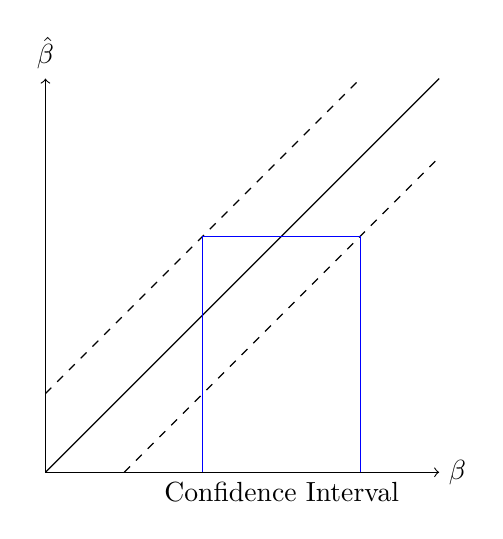
\begin{tikzpicture}
		\draw [->](0,0)--(5,0) node[right]{$\beta$};
		\draw [->](0,0)--(0,5) node[above]{$\hat{\beta}$};
		\draw (0,0)--(5,5);
		\draw[dashed] (0,1)--(4,5);
		\draw[dashed] (1,0)--(5,4);
		\draw[blue] (2,0)--(2,3);
		\draw[blue] (2,3)--(4,3);
		\draw[blue] (4,0)--(4,3);
		\draw (1,0)--(3,0) node[below]{Confidence Interval};
	\end{tikzpicture}

	What parameters could generate this estimate?
\end{frame}

\begin{frame}
	\centering
	\begin{tikzpicture}
		\draw [->](0,0)--(5,0) node[right]{$\beta$};
		\draw [->](0,0)--(0,5) node[above]{$\hat{\beta}$};
		\draw (0,0)--(5,5);
		\draw[dashed] (0,1)--(4,5);
		\draw[dashed] (1,0)--(5,4);
		\draw[blue] (2,0)--(2,3);
		\draw[blue] (2,3)--(4,3);
		\draw[blue] (4,0)--(4,3);
		\draw (1,0)--(3,0) node[below]{Confidence Interval};
		\draw[red] (0,2)--(3,2);
		\draw[red] (3,2)--(3,4);
		\draw[red] (0,4)--(3,4);
		\draw (0,1)--(0,3) node[left]{Variability of Estimator};
	\end{tikzpicture}
	
	What parameters could generate this estimate?
\end{frame}

\begin{frame}{Your Standard Error Worry}
	\begin{itemize}
		\item For hypothesis testing se tells you whether the coefficient is significant are not
		\item[]
		\item For prediction it’s telling you how variable an estimator using it really is
	\end{itemize}
\end{frame}

\begin{frame}{Dual Purpose of the Standard Error}
	\begin{itemize}
		\item The standard error also tells you that even if you’re right on average:
		
		– Your estimator will produce a lot of variance 
		
		– And then in those cases you make systematic prediction mistakes.
		\item Bias variance tradeoff
		
		– Being right on average on the coefficient is not equal to the best predictor.
	\end{itemize}
\end{frame}

\begin{frame}{The Problem Here}
	\begin{itemize}
		\item Prediction quality suffers from:
		
		– Biased coefficients
		
		– Variability in estimated coefficients
		\begin{itemize}
			\item Even if the true coefficient is 2, in any sample, we will estimate something else
		\end{itemize}
		    
		\item OLS is lexicographic
		
		– First ensure unbiased
		
		– Amongst unbiased estimators: seek efficiency
		
		\item Good predictions must trade these off
	\end{itemize}
\end{frame}

\begin{frame}{Two Variable Example}
	\begin{itemize}
		\item Belaboring the point here...		
		\item Assume now that we have two variables
		
		– As before, both normally distributed unit variance
		
		\item Your estimator produces
		$$\hat{\beta}_0^{OLS}=0\pm.2$$
		$$\hat{\beta}_1^{OLS}=2\pm10$$
	\end{itemize}
\end{frame}

\begin{frame}{What Would You Do Now?}
	\begin{itemize}
		\item Logic above suggests you would drop both variables?		
		\item[]
		\item Or keep both variables?		
		\item[]
		\item It really depends on how you feel about the variance (10)?
	\end{itemize}
\end{frame}

\begin{frame}{Calculation}
	
	\begin{align*}
		 L_n(OLS)-L_n(OLS_0)&=\overbrace{Var(\hat{\beta}_1^{OLS})+Var(\hat{\beta}_2^{OLS})}^{variance}\\
		&-\overbrace{((0-2)^2+(0-2)^2)}^{bias}\\	
		&+\underbrace{2\rho_{12}Cov(\hat{\beta}_1^{OLS},\hat{\beta}_2^{OLS})}_{covariance variance}-\underbrace{2\rho_{12}(0-2)^2}_{covariance bias}\\	
	\end{align*}
		$$L_n(OLS)-L_n(OLS_0)=\underbrace{Var(\hat{\beta}_1^{OLS})}_{variance}-\underbrace{(0-2)^2}_{bias}$$
\end{frame}

\begin{frame}{Hidden in Bias-Variance Tradeoff}
	\begin{itemize}
		\item Covariance is central
		\item[]
		\item The standard error on several variables can be large, even though together their effect is highly consistent
		\item[]
		\item For prediction covariance between x matters
	\end{itemize}
\end{frame}

\begin{frame}{In a way this problem is not important}
	$$L_n(OLS)-L_n(OLS_0)=\underbrace{Var(\hat{\beta}_1^{OLS})}_{variance}-\underbrace{(0-2)^2}_{bias}$$
	\begin{itemize}
		\item The variance term diminishes with sample size
		
		– Prediction-estimation wedge falls off as $\frac{1}{n}$
		\item But variance term increases with “variables”
		
		– Prediction-estimation rises with $k$
		
		\item So this is a problem when...
		– Function class high dimensional relative to data $\frac{k}{n}$
	\end{itemize}
\end{frame}

\begin{frame}{What this means practically}
	\begin{itemize}
		\item In some cases what you already know (estimation) is perfectly fine for prediction
		
		– This is why ML textbooks teach OLS, etc.
		
		– They are perfectly useful for the kinds of prediction problems ML tries to solve \textit{in low dimensional settings}
		\item But in high dimensional settings...
		
		– Note: high dimensional does not ONLY mean lots of variables! It can mean rich interactions.
	\end{itemize}
\end{frame}

\begin{frame}{So Far...}
	\begin{itemize}
		\item All this gives you a flavor of how the prediction task is not mechanically a consequence of the estimation task
		\item But it doesn’t really tell you how to predict 
		
		– Bias variance tradeoff is entirely unactionable 
		
		– What’s the bias?
		
		– What’s the variance?
		
		– This is not really a tradeoff you can make
		\item Adifferentlookatthesameproblemproducesa practical insight though
	\end{itemize}
\end{frame}

\begin{frame}{Back to OLS}
		$$\hat{\beta}^{OLS}=argmin_{\beta}\hat{\mathbb{E}}_{S^n}(\beta'x-y)^2$$
		$$\hat{\beta}_{prediction}^{\star}=argmin_{\beta}E_{(y,x)}(\beta'x-y)^2$$
	\begin{itemize}
		\item The real problem here is minimizing the “wrong” thing: In-sample fit vs out-of-sample fit
	\end{itemize}
\end{frame}

\begin{frame}{Overfit Problem}
	\begin{itemize}
		\item OLS looks good with the sample you have
		
		– It’s the best you can do on this sample
		\item[]
		\item Bias-variance improving predictive power is about improving out of sample predictive power
		\item[]
		\item Problem is OLS by construction overfits 
		
		– We overfit in estimation
	\end{itemize}
\end{frame}

\begin{frame}{This problem is exactly why wide data is troubling}
	\begin{itemize}
		\item Similarly think of the wide data case
		\item[]
		\item Why are we worried about having so many variables?
		\item[]
		\item We’ll fit very well (perfectly if k > n) in sample
		\item[]
		\item But arbitrarily badly out of sample
	\end{itemize}
\end{frame}

\begin{frame}{Understanding overfit}
	\begin{itemize}
		\item Let’s consider a general class of algorithms
	\end{itemize}
\end{frame}

\begin{frame}{A General Class of Algorithms}
	\begin{itemize}
		\item Let $L(f)=\int_{x,y}\ell(f(x),y)dP(x,y)$ for some loss function $l$ (e.g. squared error)
		
		– Note: $L$ is an unknown function: we don’t know $P$
		
		\item Consider algorithms of the form
		$$\hat{f}_{A,S_n}=\underset{f \in \mathcal{F}_A}{\arg\min}\hat{L}_{S_n}(f)$$
		
		– $\hat{L}_{S_n}$is used here as short hand for sample mean observations in sample $S_n$ of size $n$
		
		– OLS is an empirical loss \textit{minimizer}:it minimizes the sample average over observed data of the loss function
		
		\item So empirical loss minimization algorithms are defined by the function class they choose from
		
		\item For estimation what we typically do...
		
		– Show that empirical loss minimizers generate unbiasedness
	\end{itemize}
\end{frame}

\begin{frame}{Empirical Loss minimization}
	\begin{itemize}
		\item Leads to unbiasedness/consistency
		
		– Fit the data you have...
		
		– In a frequentist world “on average” (across all $S_{n}$) this will produce the right thing
		
		– This is usually how we prove consistency/unbiasedness
		\item[]
		\item Other variants: 
		
		– MLE
	\end{itemize}
\end{frame}

\begin{frame}{Some Notation}
	\begin{itemize}
		\item Define 
		$f^{\star}=\underset{f \in \mathcal{F}_A}{\arg\min}L(f)$ The best we can do
		$f^{\star}_A=\underset{f \in \mathcal{F}_A}{\arg\min}L(f)$ The best in the subset of functions that the algorithm looks at
		
		– Recall: L is infeasible b/c we don’t know true data- generating process
		
		\item Contrast the latter with:
		$$f_{A,S_n}=\underset{f \in \mathcal{F}_A}{\arg\min}\hat{L}_{S_n}(f)$$
		What the in-sample loss minimizer actually produces given a sample
	\end{itemize}
\end{frame}

\begin{frame}{Performance of Algorithm}
	\begin{itemize}
		\item Performance of a predictor
		$$L(\hat{f}_{A,S_n})$$	
		\item Performance of an Algorithm
		$$L_n(A) := E_{S_n}L(\hat{f}_{A,S_n})$$
		– Algorithm’s expected loss
		
		– (Suppress $S_n$ in some of the notation for estimator)
	\end{itemize}
\end{frame}

\begin{frame}{The performance of \textit{A}}
		$$L_n(A)=\underbrace{L(f^\ast)}_{\textit{irreducible error}}+\overbrace{L(f^\ast_A)-L(f^\ast)}^{\textit{approximation error}}+\boxed{\underbrace{E_{S_n}(L(\hat{f}_A)-L(f^\ast_A))}_{\textit{estimationerror}}}$$
		
		Understanding estimation error:
		
		$$E_{S_n}(L(\hat{f}_A)-L(f^\ast_A))=\overbrace{E_{S_n}(\hat{L}(\hat{f}_A)-\hat{L}(f^\ast_A))}^{\substack{\textit{"Wrong" function}\\ \textit{looks good in-sample}}}+\boxed{\underbrace{E_{S_n}(L(\hat{f}_A)-\hat{L}(\hat{f}^\ast_A))}_{\textit{Algorithm does not see this}}}$$
		
\end{frame}

\begin{frame}{Basic Tradeoff}
	\begin{itemize}
		\item These two terms go hand in hand:
			$$L_n(A)=\underbrace{L(f^\ast)}_{\textit{irreducible error}}+\boxed{\overbrace{L(f^\ast_A)-L(f^\ast)}^{\textit{approximation  error}}}+\underbrace{E_{S_n}(L(\hat{f}_A)-L(f^\ast_A))}_{\textit{estimation error}}$$
		
			$$E_{S_n}\overbrace{(L(\hat{f}_A)-L(f^\ast_A))}^{out-of-sample,\geq 0}=E_{S_n}\overbrace{(\hat{L}(\hat{f}_A)-\hat{L}(f^\ast_A))}^{in-sample,\leq 0 }+\boxed{\underbrace{E_{S_n}(L(\hat{f}_A)-\hat{L}(\hat{f}^\ast_A))}_{\textit{unseen overfit}}}$$
			
	\end{itemize}
\end{frame}

\begin{frame}{Approximation -- Overfit Tradeoff}
	\begin{itemize}
		\item If we reduce set of f to reduce possible over-fit:
		$$\underbrace{E_{S_n}(L(\hat{f}_A)-\hat{L}(\hat{f}^\ast_A))}_{\textit{unseen overfit}}$$
		\item Then we fit fewer “true functions” and drive up
		$$\overbrace{L(f^\ast_A)-L(f^\ast)}^{\textit{approximation error}}$$
		\item Only way to avoid this is if we knew information about f* so we could shrink the set
	\end{itemize}
\end{frame}

\begin{frame}{Unobserved overfit}
	\begin{itemize}
		\item So the problem of prediction really is managing unobserved overfit
		
		$$\underbrace{L(\hat{f}_A)}_{\textit{unobserved out-of-sample}}=\overbrace{\hat{L}(\hat{f}_A)}^{\textit{observed in-sample}}+\underbrace{(L(\hat{f}_A)-\hat{L}(\hat{f}_A))}_{\textit{unseen overfit}}$$
	
		\item We do well in-sample. But some of that “fit” is overfit.
\end{itemize}
\end{frame}

\begin{frame}{Return to the original example}
	\begin{columns}
		\begin{column}[t]{0.5\textwidth}
			$$OLS$$
			\qquad Greater Chance To Overfit
		\end{column}
		
		\begin{column}[t]{0.5\textwidth}
			$$OLS_0$$
			\qquad Less Chance To Overfit
		\end{column}
	\end{columns}
	
	\begin{itemize}
	\vspace{2cm}
	\item We drove down overfit by doing a constrained optimization
	\end{itemize}
\end{frame}

\begin{frame}{Basic Tradeoff at the Heart of Machine Learning}
	\begin{itemize}
		\item Bigger function classes...
		
		– The more likely we are to get to the truth (less approximation)
		
		– The more likely we are to overfit
		
		\item So we want to not just minimize in-sample error given a class of functions
		
		\item We also want to decide on the class of functions 
		
		– More expressive means less approximation error
		
		– More expressive means more overfit
	\end{itemize}
\end{frame}

\begin{frame}{Let's do the same thing here}
		Unconstrained
		$$\hat{f}_{A,S_n}=\underset{f \in \mathcal{F}_A}{\arg\min}\hat{L}_{S_n}(f)$$
		But we are worried about $\underbrace{E_{S_n}(L(\hat{f}_A)-\hat{L}(\hat{f}_A))}_{\textit{unseen overfit}}$
		
		So why not do this instead?
		$$\underset{f \in \mathcal{F}_A}{\arg\min}\hat{L}_{S_n}(f)$$
		$$ s.t.  R(f)\leq c$$ Complexity measure: tendency to overfit
\end{frame}

\begin{frame}{Return to the original example}
	\begin{columns}
		\begin{column}[t]{0.5\textwidth}
			$$OLS$$
			\qquad Greater Overfit\\ \qquad Better approximation\\ \qquad More \textbf{Expressive}\\ \qquad $R(f) higher$
		\end{column}
		
		\begin{column}[t]{0.5\textwidth}
			$$OLS_0$$
			\qquad Less Overfit\\ \qquad Worse approximation\\ \qquad Less \textbf{Expressive}\\ \qquad $R(f) lower$
		\end{column}
	\end{columns}
	
	\begin{itemize}
		\vspace{1cm}
		\item Reduce overfit by approximating worse
		\item Choose less expressive function class
	\end{itemize}
\end{frame}

\begin{frame}{Constrained minimization}
	\begin{itemize}
		\item We could do a constrained minimization
		\item But notice that this is equivalent to:
		$$\hat{f}_{A_\lambda,S_n}=\underset{f \in \mathcal{F}_A}{\arg\min}\hat{L}_{S_n}(f)+\underbrace{\lambda R(f)}_{want:\approx L(f)-\hat{L}(f)}$$
		
		
		\item Complexity measure should capture tendency to overfit
	\end{itemize}
\end{frame}

\begin{frame}{Basic insight}
	\begin{itemize}
		\item Data has signal and noise
		\item[]
		\item More expressive function classes
		
		– Allow us to pick up more of the signal 
		
		– But also pick up more of the noise
		\item[]
		\item So the problem of prediction becomes the problem of \textit{choosing expressiveness}
	\end{itemize}
\end{frame}

\begin{frame}{Overall Structure}
	\begin{itemize}
		\item Create a regularizer that:
		
		– Measures expressiveness
		\item[]
		\item Penalize algorithm for choosing more expressive functions
		
		– Tuning parameter lambda
		\item[]		
		\item Let it weigh this penalty against in-sample fit
	\end{itemize}
\end{frame}

\begin{frame}{Liner Example}
	\begin{itemize}
		\item Linear function class $x \rightarrow \beta'x (\beta \in \mathbb{R}^{k+1})$
		\item[]
		\item Regularized linear regression
		$$\hat{\beta}_\lambda^R=\underset{\beta \in \mathbb{R}^{k+1}}{\arg\min}\hat{\mathbb{E}}_{S_n}(\beta'x-y)^2-\lambda R(\beta)$$
	\end{itemize}
\end{frame}

\begin{frame}{Regularizers for Linear Functions}
	\begin{itemize}
		\item Linear functions more expressive if use more variables
		$$R(\beta)=\sum_{j=1}^{k}1_{\beta_j}\neq 0$$
		
		\item Can transform coefficients
		$$R(\beta)=\sum_{j=1}^{k}|\beta_j|^p$$
	\end{itemize}
\end{frame}

\begin{frame}{Computationally More Tractable}
	\begin{columns}
		\begin{column}{0.4\textwidth}
		\begin{itemize}
		\item Lasso
		$$\mathcal{F}_{1,c}=\{f_\gamma; \sum_{j=1}^{k}|\gamma_j|\leq c\}$$
		\item Ridge
		$$\mathcal{F}_{2,c}=\{f_\gamma; \sum_{j=1}^{k} \gamma_j^2\leq c\}$$
		\end{itemize}
		\end{column}
		
		\begin{column}{0.6\textwidth}
				\begin{tikzpicture}
				\draw [red](3,3) circle(2);
			\end{tikzpicture}
		\end{column}
	\end{columns}
\end{frame}

\begin{frame}{What makes a good regularizer?}
	\begin{itemize}
		\item You might think...
		
		– Bayesian assumptions 
		
		– Example: Ridge
		\item A good regularizer can build in beliefs
		\item Those are great and useful when available
		\item But central force is tendency to overfit
		\item Example:
		
		– Even if true world were not sparse or priors were not normal you’d still do this
	\end{itemize}
\end{frame}

\begin{frame}{Summary}
	\begin{itemize}
		\item Regularization is one half of the secret sauce
		\item[]
		\item Gives a single-dimensional way of deciding of capturing expressiveness
			$$\hat{f}_{A_\lambda,S_n}=\underset{f \in \mathcal{F}_A}{\arg\min}\hat{L}_{S_n}(f)+\lambda R(f)$$		
		\item[]	
		\item Still missing ingredient is lambda
	\end{itemize}
\end{frame}

\begin{frame}{Choosing lambda}
	\begin{itemize}
		\item How much should we penalize expressiveness?
		\item[]
		\item How do you make the over-fit approximation tradeoff?	
		\item[]
		\item The \textbf{tuning} problem.
		\item[]
		\item Use cross-validation
	\end{itemize}
\end{frame}

\begin{frame}{How Does Cross Validation Work?}
		Tuning Set = 1/5 of Training Set
\end{frame}

\begin{frame}{Cross-Validation Mechanics}
	\begin{itemize}
		\item Loop over cross-validation samples
		
		– Train a deep tree on CV-training subset
		\item[]
		\item Loop over penalty parameters $\lambda$
		
		– Loop over cross-validation samples 
		\begin{itemize}
			\item Prune the tree according to penalty
			\item Calculate new MSE of tree
		\end{itemize}
		
		– Average (over c-v samples) the MSE for this penalty
		\item[]
		\item Choose the penalty $\lambda^\star$ that gives the best average MSE
	\end{itemize}
\end{frame}

\begin{frame}{LASSO c-v Example}
	
\end{frame}

\begin{frame}{Creating Out-of-Sample \textbf{In Sample}}
	\begin{itemize}
		\item Major point:
		
		– Not many assumptions
		
		– Don’t need to know true model.
		
		– Don’t need to know much about algorithm
		\item Minor but important point
		
		– To get asymptotics right we need to make some regularity assumptions
		\item Side point (to which we return)
		
		– We’d like to choose best algorithm for sample size n 
		
		– But this will not do that. Why?
	\end{itemize}
\end{frame}

\begin{frame}{Why does this work?}	
	\begin{enumerate}
		\item Not just because we can split a sample and call it out of sample
		
			– It’s because the thing we are optimizing is \textbf{observable} (easily estimable)
	\end{enumerate}
\end{frame}

\begin{frame}{This is more than a trick}
	\begin{itemize}
		\item It illustrates what separates prediction from estimation:
		
		– I can’t ‘observe’ my prior.
		\begin{itemize}
			\item Whether the world is truly drawn from a linear model
		\end{itemize}
		
		– But prediction quality is observable
		\item Put simply:
		
		– Validity of predictions are measurable
		
		– Validity of coefficient estimators require structural knowledge
	\end{itemize}
	\textit{This is the essential ingredient to prediction: Prediction quality is an empirical quantity not a theoretical guarantee}
\end{frame}

\begin{frame}{Why does this work?}	
	\begin{enumerate}
		\item It’s because the thing we are optimizing is \textbf{observable} \vspace*{0.5cm}
		\item By focusing on prediction quality we have \textbf{reduced dimensionality}
	\end{enumerate}
\end{frame}

\begin{frame}{To understand this...}
	\begin{itemize}
		\item Suppose you tried to use this to choose coefficients
		\begin{itemize}
			\item Ask which set of coefficients worked well out-of sample.
		\end{itemize}
		\item Doesthiswork?
		\item Problem1: Estimation quality is unobservable
		\begin{itemize}
			\item Need the same assumptions as algorithm to know whether you “work” out of sample
			\item If you just go by fit you are ceding to say you want best predicting model
		\end{itemize}
		\item Problem 2: No dimensionality reduction.
		\begin{itemize}
			\item You’ve got as many coefficients as before to search over
		\end{itemize}
	\end{itemize}
\end{frame}

\begin{frame}
		$$\hat{\beta}_\lambda^R=\underset{\beta \in \mathbb{R}^{k+1}}{\arg\min}\mathbb{E}_{S_n}(\beta'x-y)^2-\lambda R(\beta)$$
		
		\centering
		\begin{tabular}{cc}
			\toprule
			Method&$R(\beta)$\\
			\midrule
			OLS&0\\
			Subset selection&$||\beta||_0=\sum_{j=1}^{k}\mathcal{1}_{\beta_j\neq 0}$\\
			Lasso&$||\beta||_1=\sum_{j=1}^{k}|\beta_j|$\\
			Ridge&$||\beta||_2^2=\sum_{j=1}^{k}\beta_j^2$\\
			Elastic Net&$\alpha||\beta||_1+(1-\alpha)||\beta||^2_2$\\
			\bottomrule
		\end{tabular}
\end{frame}

\begin{frame}{Bayesian Interpretation of Ridge}
Consider the regression
$$Y_i=\sum_{k=1}^{K}\beta_kX_{ik}+\varepsilon_i$$
with
$$\varepsilon_i|X_{i1},...,X_{iK}\sim N(0,\sigma^2)$$
suppose we put a prior on the $\beta_k$ :
$$\beta_k\sim N(0,\tau^2)$$
and all the $\beta_k$ independent. Assume $\sigma^2$ is known.
\end{frame}

\begin{frame}{Bayesian Interpretation of Ridge}
	Then the posterior distribution is proportional to
	\begin{align*}
		p(\beta|data)&\propto \exp\left(-\frac{1}{2\sigma^2}\sum_{j=1}^{N}\left(Y_i-\sum_{k=1}^{K}\beta_kX_ik\right)^2\right)\prod\limits_{k=1}^K\exp\left(-\frac{\beta^2_k}{2\tau^2}\right)\\
		&=\exp\left(-\frac{1}{2\sigma^2}\sum_{j=1}^{N}\left(Y_i-\sum_{k=1}^{K}\beta_kX_ik\right)^2-\sum_{k=1}^{K}\frac{\beta^2_k}{2\tau^2}\right)\\
		&=\exp\left(-\frac{1}{2\sigma^2}\sum_{j=1}^{N}(Y_i-\beta'X_i)^2-\frac{\beta'\beta}{2\tau^2}\right)\\
	\end{align*}
\end{frame}

\begin{frame}{Bayesian Interpretation of Ridge}
	So, the posterior is normal, and the posterior mean minimizes
	\begin{align*}
		\sum_{i=1}^{N}&(Y_i-\beta'X_i)^2+\beta'\beta\frac{\sigma^2}{\tau^2}\\
		&=\sum_{i=1}^{N}(Y_i-\beta'X_i)^2+\frac{\sigma^2}{\tau^2}||\beta||^2\\
	\end{align*}
	This leads to the posterior mean
	$$\left( \X^{'}\X+I_K\cdot\sigma^2/\tau^2\right) ^{-1}\X^{'}\Y.$$
	If the $\X^{'}\X$ matrix is diagnoal, all elements of $\beta$ would be shrunk
	towards zero by the same fraction. WIth a non-diagonal matrix the degree of
	shrinkage vaires.
\end{frame}

\begin{frame}{POST Lasso}
	\begin{itemize}
		\item Important distinction:
		
		– Use LASSO to choose variables 
		
		– Use OLS on these variables
		\item[]
		\item How should we think about these?
	\end{itemize}
\end{frame}

\begin{frame}
	
\end{frame}

\begin{frame}
	In the orthonormal case, i.e. $\X^{'}\X=\mathbf{I}=(\X^{'}\X)^{-1}$:
	$$\hat{\beta}_j(\lambda_1)=sgn(\hat{\beta}_j)(|\hat{\beta}_j|-\lambda_1/2)_+$$
		\begin{columns}
		\begin{column}{0.4\textwidth}
		That is, the lasso estimate is related to the OLS estimate via the so-called {\color{blue}soft threshold function} (depicted here for $\lambda_1$).
		\end{column}
		
		\begin{column}{0.6\textwidth}

		\end{column}
	\end{columns}
\end{frame}

\begin{frame}{Why not Hard Thresholding?}
	\centering Soft Thresholding
	\begin{tikzpicture}
		\draw [->](0,0)--(6,0) node[right]{$\hat{\beta}_{OLS}$};
		\draw [->](0,0)--(0,6) node[above]{$\hat{\beta}_{LASSO}$};
		\draw[dashed] (0,0)--(6,6);
		\draw[blue] (0,1)--(2,3);
		\draw[blue] (4,3)--(6,5);
		\draw[red] (2,3)--(4,3);
		\draw[red] (0,0)--(2,2);
		\draw[red] (4,4)--(6,6);
	\end{tikzpicture}
\end{frame}

\begin{frame}
	\centering	
	Orthonormal: $\hat{\beta}_{RIDGE}=\frac{\hat{\beta}_{OLS}}{1+\lambda}$

	\begin{tikzpicture}
		\draw [->](0,0)--(4,0) node[right]{$\hat{\beta}_{OLS}$};
		\draw [->](0,0)--(0,4) node[above]{$\hat{\beta}_{RIDGE}$};
		\draw[dashed] (0,0)--(4,4);
		\draw[blue] (0,0)--(4,2);
	\end{tikzpicture}
\end{frame}

\begin{frame}
	\begin{columns}
		\begin{column}{0.5\textwidth}
	\begin{tikzpicture}
	\draw [->](0,0)--(4,0) node[right]{$\hat{\beta}_{OLS}$};
	\draw [->](0,0)--(0,4) node[above]{$\hat{\beta}_{LASSO}$};
	\draw[dashed] (0,0)--(4,4);
	\draw[blue] (0,2/3)--(4/3,2);
	\draw[blue] (8/3,2)--(4,10/3);
	\draw[blue] (4/3,2)--(8/3,2);
\end{tikzpicture}
		\end{column}
		
		\begin{column}{0.5\textwidth}
			\begin{tikzpicture}
				\draw [->](0,0)--(4,0) node[right]{$\hat{\beta}_{OLS}$};
				\draw [->](0,0)--(0,4) node[above]{$\hat{\beta}_{RIDGE}$};
				\draw[dashed] (0,0)--(4,4);
				\draw[blue] (0,0)--(4,2);
			\end{tikzpicture}
		\end{column}
	\end{columns}
\vspace*{1cm}
\centering Can be very misleading
\end{frame}


\end{document}







